\chapter{Kryptologie}

\section{Grundbegriffe und einfache Verfahren}
\begin{figure}[h]
	\centering
	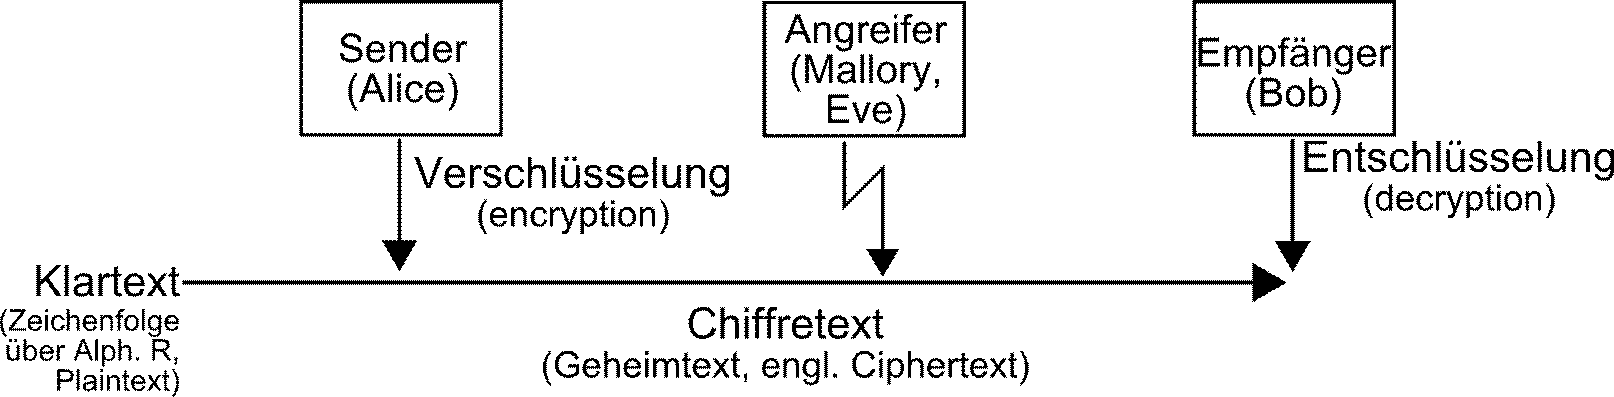
\includegraphics[width=15cm]{./img/krypto_schaubild.png}
	\caption{Schaubild der Kryptologie}
	\label{img:Schaubild Kryptologie}
\end{figure}

\subsection{Verschl\"usselung erfordert}

\begin{itemize}
	\item[-] Verschl\"usselungsverfahren, Algorithmus (Funktion)
	\item[-] Schl\"ussel $k_{e}$ (encryption key)
\end{itemize}

\[
	E(m,k_e)=c
\]	
$E$=Verschl\"usselungs Funktion, $m$=Klartext, $c$=Chiffretext
\[
	E(m_1,k_e) \neq E(m,k_e) \text{ f\"ur }m_1 \neq m_2
\]
\[
	D(c,k_d)=m
\]	
($k_d$ zu $k_e$ geh\"origer Dechiffrierschl\"ussel!)\\
$k_d=k_e$ (oder $k_d$ leicht aus $k_e$ zu berechnen):\\
\textbf{symmetrisches Verschl.verf.}, ansonsten \textbf{asymm. Verschl.verf.}. Ist $k_d$ nur sehr schwer (oder garnicht) zu $k_e$ berechenbar, so kann $k_e$ ver\"offentl. werden:\\
\textbf{Public-Key-Verfahren}.

\subsection{Beispiel f\"ur (nicht sicheres) symm. Verfahren}

\begin{itemize}
	\item[a)] $R=S=\left\{0,1,\ldots,25\right\}$\\
	Verfahren: Verschiebechiffre\\
	Schl\"ussel: $i \in \left\{0,1,\ldots,25\right\}$\\
	Verfahren $ x \in \R \longrightarrow x+i \mod{26}=y$\\
	$y\longmapsto y-i \mod{26} = y$\\
	$m=x_1 ... x_2 \longrightarrow  c = (x_1 + i \mod{26}) \textbf{}\ldots (x_n +i \mod{26})$, $E(m,i)$\\
	Unsicher, weil Schl\"usselmenge klein ist (Brute Force Angriff).
	\item[b)] R,S, Schl\"usselmenge=Menge aller Permutationen von $\left\{1,\ldots,25\right\}=S_{26}$\\
	Verschl.: W\"ahle Permuation $\pi$\\
	$x \in \R \longrightarrow \pi (x)=y$\\
	Entschl.: $y \longrightarrow \pi^{-1}(y)=x$\\
	$m=x_1 \ldots x_r \rightarrow c=\pi(x_1)\ldots\pi(x_r)$\\
	$\begin{pmatrix}
  0 & 1 & 2 & \ldots & 25 \\
  3 & 17 & 4 & \ldots & 13
	\end{pmatrix}
	\longrightarrow \pi(0)=3$, u.s.w.\\
	Anzahl der Permutationen: $\left|{S_{26}}\right|=26!\approx4\cdot10^{26} \longrightarrow$ Brute-Force Angriff nicht mehr m\"oglich! \\
	Warum? Man muss im Schnitt 50\% der Permutationen testen. Angenommen man k\"onnte $10^12$ Perm. pro Sekunde testen.\\
	Aufwand: $2\cdot10^{14}$ Sekunden $\approx 6.000.000$ Jahre\\
	Trotzdem unsicher!\\
	Grund: Charakteristiches H\"aufigkeitsverteilung von Buchstaben in nat\"urlichspr. Texten.
\end{itemize}
Verfahren beinhalten viele Verschl\"usselungsm\"oglichkeiten, abh\"angig von der Auswahl des Schl\"ussels.\\
Verfahren bekannt, aber Schl\"ussel $k_d$ geheim!\\
\subsection{Prinzip von Kerkhoffs (1835-1903)}
Sicherheit eines Verschl\"usselungsverfahren darf nicht von der Geheimhaltung des Verfahrens, sondern nur von der Geheimhaltung des verwendeten Schl\"ussels abh\"angen!
%
%	Ende Stunde vom 29.10.2009
%
\\\\
Kryptologie besteht aus Kryptographie (Entwurf) und der Kryptoanalyse (Angriff).
Angriffserfolge:
\begin{itemize}
	\item[-] Schl\"ussel $k_d$ wird gefunden
	\item[-] Eine zu der Dechiffrierfunktion $D(\cdot,k_d)$ \"aquivalente Funktion finden ohne Kenntnis von $k_d$
	\item[-] gewisste Chiffretexte werden entschl\"usselt
\end{itemize}
\subsection{Arten von Angriffen}
\begin{itemize}
	\item[-] Ciphertext-Only Angriff
	\item[-] Known-Plaintext Angriff
	\item[-] Chosen-Plaintext Angriff
	\item[-] Chosen-Ciphertext Angriff
\end{itemize}


%p2
\section{One-Time-Pad und perfekte Sicherheit}

Lauftextverschl\"usselung\\
\\
Alphabet $\Z_k=\{0,1,\ldots,k-1\}$\\
In $\Z_k$ kann man addieren und multiplizieren mit $\md{k}$.\\
\\
Klartext $x_1,x_2,\ldots,x_n$\\
Schl\"usselwort $k_1,k_2,\ldots,k_n$\\
$x_1 + k_1 \mod{k}$, $x_n + k_n \mod{k} \leftarrow$ Chiffretext\\
\\
Mit nat\"urlichsprachlichen Texten ist das Verfahren unsicher.\\
$\Z_2=\{0,1\}$, $1 \oplus 1 = 0 = 0 \oplus 0$, $0 \oplus 1 = 1 = 1 \oplus 0 \Rightarrow XOR$\\
Klartext in $\Z_2^n=\{(x_1,\ldots,x_n):x_i \in \Z_2\}$
Schl\"ussel: Zufallsfolge \"uber $\Z_2$ der L\"ange $n$. $m$ Klartext, $k$ Zufallsfolge (beide L\"ange $n$)
\[
	c=m\oplus k, (x_1,\ldots,x_n)\oplus(k_1,\ldots,k_n):=(x_1\oplus k_1,\ldots,x_n\oplus k_n)
\]
\subsection{One-Time-Pad}
Schl\"ussel $k$ darf nur einmal verwendet werden!\\
\[
	m_1\oplus k=c_1, m_2 \oplus k=c_2,c_1\oplus c_2=m_1\oplus k \oplus m_2\oplus k=m_1\oplus m_2
\]
Wieder nur Lauftext $\rightarrow$ unsicher!\\
$m_1$ und $m_2$ l\"asst sich ermitteln.\\
Zufallsfolge der L\"ange $n$: eigentlich unsinniger Begriff. Da jedes Bit unabh\"angig von anderen mit Wahrscheinlichkeit $\frac{1}{2}$ erzeugt wird (Output einer bin\"ar symmetrischen Quelle)\\
Jede Folge der L\"ange $n$ ist gleich wahrscheinlich (Wahrscheinlichkeit $\frac{1}{2} n$\\
One-Time-Pad ist perfekt sicher.
\subsection{Perfekte Sicherheit}
Ein Verschl\"usselungsverfahren ist perfekt sicher, falls gilt: F\"ur jeden Klartext $m$ und jedem Chiffretext $c$ (der festen L\"ange $n$)
\[
	pr(m|c)=pr(m)
\]
$pr(m|c)\rightarrow$ A-posteriori-Wahrscheinlichkeit (Wahrscheinlichkeit, dass $m$ Klartext, wenn $c$ empfangen wurde)\\
$pr(m)\rightarrow$ A-priori-Wahrscheinlichkeit\\
\\
\textbf{Beispiel:} Substitutionschiffre aus Kapitel 2.\\
$n=5, m=HALLO, pr(m)>0$\\
Ang:$c=QITUA$ wird empfangen, $LL\neq TU \rightarrow pr(m|c)=0$\\
nicht perfekt sicher.\\
\\
One-Time-Pad ist perfekt sicher. \\
(Bayes'sche Formel) $m\oplus k$\\
Jede Folge $c$ l\"asst sich mit geeignetem $k$ in der Form $c=m\oplus k$ erhalten.\\
W\"ahle $k=m\oplus c$, $m\oplus k=m\oplus m \oplus c=c$\\
Bei gegebenem $m$ und zuf\"allige gew\"ahlten Schl\"ussel $k$ ist jeder Chiffretext gleichwertig.

%p3

\section{Symmetrische Blockchiffre}
\subsection{Blockchiffre}
Zerlege Klartext in Bl\"ocke (Strings) der L\"ange $n$.  Jeder Block wird einzeln verschl\"usselt (in der Regel wieder in einem Block der L\"ange $n$). Gleiche Bl\"ocke werden gleich verschl\"usselt.\\
\\
Wieviele Blockchiffren der L\"ange $n$ gibt es?\\
Alphabet $\Z_2=\{0,1\}$\\
$|\{\underbrace{(0,\ldots,0)}_{Block},(0,\ldots,1),\ldots,(1,\ldots,1)\}| = 2^n$\\
Blockchiffre = Permuation der $2^n$ Bl\"ocke.\\
$(2^n)!$ Blockchiffre\\
\\
Wenn alle verwendet werden:\\
Schl\"ussel = Permuation der $2^n$ Bl\"ocke\\
$(x_{1,1},\ldots,x_{1,n},x_{2,1},\ldots,x_{2,n},\ldots)$ \ \ \fbox{$n\cdot 2^n$ Bit}\\
Zur Speicherung eines Schl\"ussels werden $n \cdot 2^n$ Bit ben\"otigt.\\
Zum Beispiel:\\
$n=64, \ 64 \cdot 2^{64}=2^{70}\approx$ 1 ZetaByte $\approx$ 1 Milliarde Festplatten � 1 TB\\
\textbf{Illusional!}\\
\\
Konsequenz:\ Verwende Verfahren, wo nur ein kleiner Teil der Permutation als Schl\"ussel verwendet wird und so sich die Schl\"ussel dann in k\"urzerer Fom darstellt.
%
% Ende zweiter Vorlesung
%

%p4
\subsection{Vorbemerkung}

\subsubsection{$n\times m$-Matrix}

\[
\begin{pmatrix}
	a_{11} & \ldots & a_{1m} \\
	\vdots &  & \vdots \\
	a_{n1} & \ldots & a_{nm}
\end{pmatrix}
\]

$1 \times n$ = Zeilenvektor = $(a_1,\ldots,a_m)$

$n \times 1$ = Spaltenvektor = $\begin{pmatrix} b_1 \\ \vdots \\ b_n \end{pmatrix}$

z.B. $a_{ij} \in \R,\ a_{ij} \in \Z$ oder $a_{ij} \in R,\ R$ Ring

$n \times m$-Matrix A,B
\[
\begin{pmatrix}
	a_{11} & \ldots & a_{1m} \\
	\vdots &  & \vdots \\
	a_{n1} & \ldots & a_{nm}
\end{pmatrix}
+
\begin{pmatrix}
	b_{11} & \ldots & b_{1m} \\
	\vdots &  & \vdots \\
	b_{n1} & \ldots & b_{nm}
\end{pmatrix}
:=
\begin{pmatrix}
	a_{11}+b_{11} & \ldots & a_{1m}+b_{1m} \\
	\vdots &  & \vdots \\
	a_{n1}+b_{n1} & \ldots & a_{nm}+b_{nm}
\end{pmatrix}
\]
\[
A=n\times m,\ B = m \times k,
\]
\[
A \cdot B
\begin{pmatrix}
	c_{1l} & \ldots & c_{1k} \\
	\vdots &  & \vdots \\
	c_{m1} & \ldots & c_{mk}
\end{pmatrix}
=
n\times k
\]
\[
c_{1l}=(a_{i1} \cdot b_{ij})+(a_{i2} \cdot b_{2j}) + \ldots + (a_{im} \cdot b_{mj})
\]
\[
(A+B)\cdot C = A\cdot B + B\cot C
\]

Im Allgemeinem: $A\cdot B \neq B\cdot A$\\

\subsubsection{Quadritsche Matrix ($n\times n$)}

\[
E_n=\begin{pmatrix}
	1 & \ldots & 0 \\
	\vdots & \ddots & \vdots \\
	0 & \ldots & 1
\end{pmatrix}
\]
\[
A=n\times n,\ A \cdot E_n=E_n \cdot A = A
\]
$A\ n\times n$-Matrix \"uber kommutativen Ring R mit Eins.\\
Wann existiert Matrix $A^{-1}$(Inverse Matrix) mit $A^{-1} \cdot A = A \cdot A^{-1} = E_n$?\\
$det(A) \in R$\ Determinante von A\\
\\
$2\times 2$-Matrix: $det\begin{pmatrix}
	a_{11} & a_{12} \\ a_{21} & a_{21}
\end{pmatrix}
= a_{11} \cdot a_{22} - a_{12} \cdot a_{21}$\\
\\
\\
A besitzt inverse Matrix $\Leftrightarrow det(A)$ in R ein inverses besitzt\\
(z.B. R K\"orper, $\Z ,\Q ,\Z_p,\ det(A)\neq 0$\\
\[
A^{-1}=
\begin{pmatrix}
	\frac{1}{det(A)}\cdot b_{11} & \ldots & \frac{1}{det(A)}\cdot b_{1m} \\
	\vdots & & \vdots \\
	\frac{1}{det(A)}\cdot b_{n1} & \ldots & \frac{1}{det(A)}\cdot b_{nm}
\end{pmatrix}
\]
$b_{ij}=(-1)^{i+j}$\ $det(A_{ji})$\\
\\
$A_{ji}=(n-1)\times (n-1)$-Matrix, die aus $A$ durchstreichen der $j$-ten Zeile und $i$-ten Spalte entsteht.
\[
A=
\begin{pmatrix}
	a_{11} & a_{12} \\ a_{21} & a_{22}
\end{pmatrix}\ \
A^{-1}=
\begin{pmatrix}
	a_{22} & -a_{12} \\ -a_{21} & a_{11}
\end{pmatrix}
\]
$R=\Z_k \ \{0,1,\ldots,k\}$\\
Addition und Multiplikation in $\Z_k (\oplus,\odot)$\\
normale Add. und Mult. mit $\md{k}$\\

\subsection{Affin-lineare Chiffren}
Klartextalphabet = Chiffretextalphabet = $\Z_k$ ($k=2,\ k=26$)\\
W\"ahle $n \times n$-Matrix $A$ \"uber $\Z_k$ und Zeilenvektor $b$ der L\"ange $n$ \"uber $\Z_k$. Dies wird der Schl\"ussel sein f\"ur die Chiffrierung.\\
Blockchiffre der L\"ange $n$. \\
Block = Zeilenvektor der L\"ange $n$ \"uber $\Z_k$. \\
Klartextblock $v$\\
Chiffretextblock
\begin{align*}
	v \cdot A + b &=: w\\
	v \rightarrow v \cdot A +b &=:w\\
	w-b&=v \cdot A
\end{align*}	
ben\"otigen: $A^{-1}$ existiert (d.h. $ggT(det(A),k)=1$)\\
Dechiffrierung:
\[
	(w-b)\cdot A^{-1} = v \cdot A \cdot A^{-1} = v \cdot E_n = v
\]
(wenn immer b=0 gew\"ahlt wird, dann lineare Chiffren, Hill-Chiffren)\\
Beispiel:\\
\[
	A=
	\begin{pmatrix}
		1 & 3 \\ 3 & 2
	\end{pmatrix},
	\quad Z_6
\]
Blockchiffre der L\"ange $n$
$det(A)=1 \cdot 2 - 3 \cdot 3 = -7 = 5$ inverse in $\Z_6$
\begin{align*}
	\frac{1}{det(A)}&=det(A)^{-1}=5 \\
	A^{-1}=5\cdot
	\begin{pmatrix}
		2&-3\\-3&1
	\end{pmatrix}
	&=
	\begin{pmatrix}
		10&-15\\-15&5
	\end{pmatrix}
	=
	\begin{pmatrix}
		4&3\\3&5
	\end{pmatrix}
\intertext{Test:}
	A \cdot A^{-1} = 
	\begin{pmatrix}
		1 & 3 \\ 3 & 2
	\end{pmatrix}
	\cdot
	\begin{pmatrix}
		4&3\\3&5
	\end{pmatrix}
	&=
	\begin{pmatrix}
		4+9&3+15\\12+6&9+10
	\end{pmatrix}
	=
	\begin{pmatrix}
		1&0\\0&1
	\end{pmatrix}
\end{align*}
Verschl\"usselung:
Schl\"ussel:
\[
	A = 
	\begin{pmatrix}
		1 & 3 \\ 3 & 2
	\end{pmatrix}\\
	\quad b=(3,5)
\]	
Klartextblock: $(1,2)$\\
Chiffretextblock: 
\begin{align*}	
	w&=(1,2) \cdot 
	\begin{pmatrix}
		1 & 3 \\ 3 & 2
	\end{pmatrix}
	+
	(3,5)= (1,1)+(3,5) = (4,0)
\intertext{Entschl\"usselung:}
	(w-b) \cdot A^{-1} &= (1,1) \cdot 
	\begin{pmatrix}
		4 & 3 \\ 3 & 5
	\end{pmatrix}
	=(1,2)
\end{align*}
$\Z_2 : n^2 + n$ Bit zur Speicherung eines Schl\"ussels.\\
Wieviele inverse Matrizen \"uber $\Z_2$ mit $n=64$?
\[
	(2^{64}-1) \cdot (2^{64}-2) \cdot \ldots \cdot (2^{64}-2^{63}) \approx 0.29 \cdot 2^{4096}
\]
Verfahren ist unsicher gegen\"uber Known-Plaintext-Angriffe.\\
$(A,b)$ Schl\"ussel, A inverse $n \times n$-Matrix \"uber $\Z_k ,b \ \in \Z_k^n$\\
Angenommen Angreifer kennt $n+1$ Klartext/Chiffretextpaare verschl\"usselt mit $(A,b),\ v_0, v_1,\ldots,v_n \ w_0,\ldots,w_n$\\
Dann kann er haufig $(A,b)$ bestimmen.
\[
	V=
	\begin{pmatrix}
		v_1-v_0\\v_2-v_0\\\vdots\\v_n-v_0
	\end{pmatrix}
	\ n \times n-\text{Matrix}
\]	

Angenommen: V ist invertierbar. Setze $W=
\begin{pmatrix}
	w_1-w_0\\\vdots\\w_n-w_0
\end{pmatrix}$
\[
V \cdot A =
\begin{pmatrix}
	(v_1-v_0) \cdot A \\ \vdots \\(v_n-v_0) \cdot A
\end{pmatrix}
=
\begin{pmatrix}
	v_1 \cdot A + b - v_0 \cdot A +b \\ \vdots \\
	v_n \cdot A + b - v_0 \cdot A + b
\end{pmatrix}
=
\begin{pmatrix}
	w_1-w_0\\ \vdots\\w_n-w_0
\end{pmatrix}
=W
\]

$V \cdot A$ bekannt, also auch $V^{-1}$:

$A=V^{-1} \cdot w$

$b=w_0 - v_0 \cdot A$

Beispiel: $n=2,\ k=25 \ \ \{A,\ldots, Z\}=\{0,\ldots,25\}$

\begin{center}
\texttt{HERBST} $\longrightarrow$ \texttt{NEBLIG}

\begin{tabular}{l|l|l}
H & 7 & \multirow{2}{*}{$v_0$} \\
E & 4 & \\
\hline
R & 17 & \multirow{2}{*}{$v_1$} \\
B & 1 & \\
\hline
S & 18 & \multirow{2}{*}{$v_2$} \\
T & 19 &
\end{tabular}
$\longrightarrow$
\begin{tabular}{l|l|l}
N & 13 & \multirow{2}{*}{$w_0$} \\
E & 4 & \\
\hline
B & 1 & \multirow{2}{*}{$w_1$} \\
L & 11 & \\
\hline
I & 8 & \multirow{2}{*}{$w_2$} \\
G & 6 &
\end{tabular}
\end{center}
\begin{align*}
	V&=
	\begin{pmatrix}
		10 & -3 \\
		11 & 15
	\end{pmatrix}
	=
	\begin{pmatrix}
		10 & 23\\
		11 & 15
	\end{pmatrix}, \quad
	W=
	\begin{pmatrix}
		14 & 7 \\
		21 & 2
	\end{pmatrix}\\
	det(V) &= 10 \cdot 15  + 33 = 183 \equiv 1 (\md{26})\\
	V^{-1}&=
	\begin{pmatrix}
		15 & 3 \\
		-11 & 10 	
	\end{pmatrix}
	=
	\begin{pmatrix}
		15 & 3 \\
		15 & 10 	
	\end{pmatrix}\\
	A&=V^{-1} \cdot W =
	\begin{pmatrix}
		15 & 3 \\
		15 & 10 	
	\end{pmatrix}
	\cdot
	\begin{pmatrix}
		14 & 7 \\
		21 & 2
	\end{pmatrix}
	=
	\begin{pmatrix}
		210+63 & 105+6 \\
		210+210 & 105+20
	\end{pmatrix}
	=
	\begin{pmatrix}
		13 & 7\\
		4 & 21
	\end{pmatrix}\\
	b&=w_0-v_0 \cdot A = (13,4) - (7,4) \cdot 
	\begin{pmatrix}
		13 & 7\\
		4 & 21
	\end{pmatrix}
	=
	(10,1)
\intertext{Test:}
	v_1 &\cdot A + b = w_1,\quad v_2 \cdot A + b= w_2
\end{align*}

%p5

\section{Der Advanced Encryption Standard (AES)}
\subsection{Mathematische Methoden gebraucht f\"ur AES} % NEED BETTER TITLE HERE
Seit 70er Jahren gab es DES (Blockl\"ange 64 Bit, Schl\"ussell\"ange 56 Bit) \\
\\
Nachfolger des DES: Daemen, Rijmen (Belgier)\\
Rijndael-Verfahren $\rightarrow$ AES (2002 FIPS 197)\\
\\
Iterierte Blockchiffre\\
Version mit 128 Bit Block und Schl\"ussel\"ange. \\
\begin{figure}[ht]
	\centering
	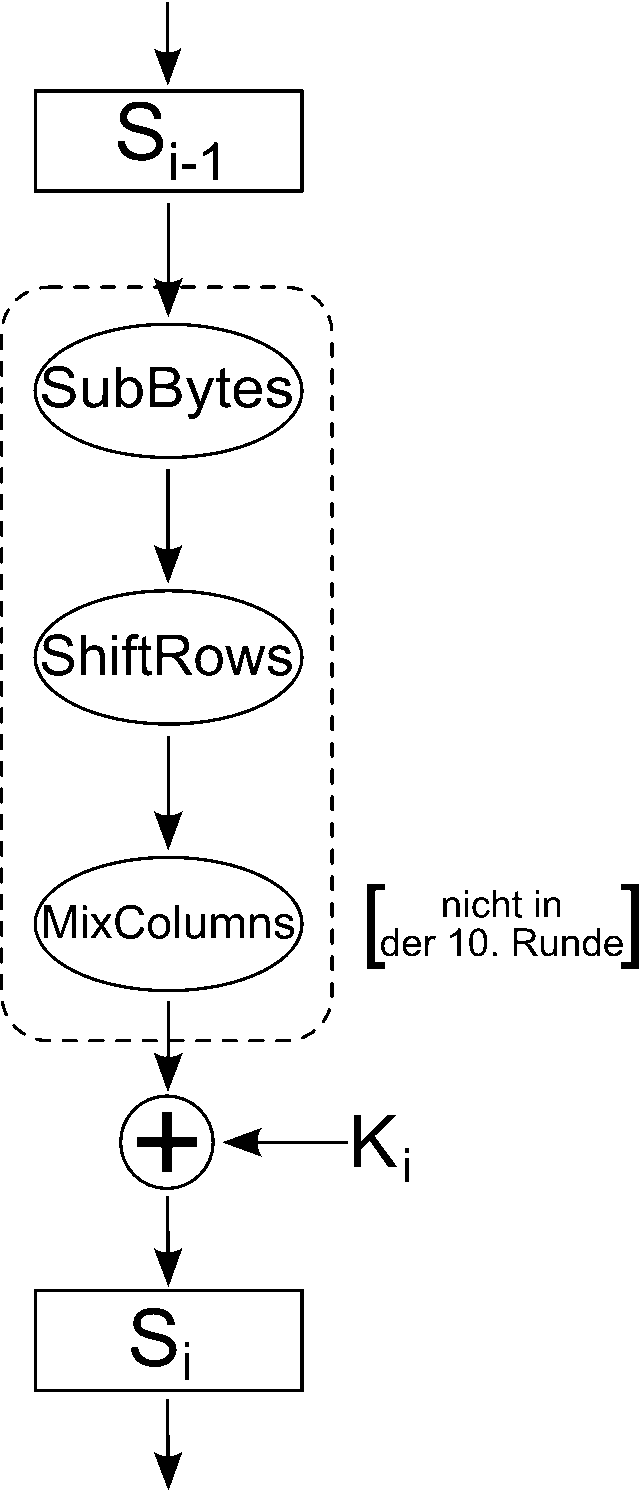
\includegraphics[height=8cm]{./img/AES_round.png}
	\caption{Eine Runde vom AES}
	\label{img:Eine Runde vom AES}
\end{figure}Vorbemerkung: 128-Bit Bl\"ocke werden dargestellt als:\\
\[
	\begin{pmatrix}
		a_{01} & a_{02} & \ldots & a_{03} \\
		a_{10} & a_{11} & \ldots & a_{13}\\
		\vdots & \vdots  & \vdots & \vdots \\
		a_{30} & \ldots  & \ldots & a_{33}
	\end{pmatrix}
\]
Jedes $a_{ij}$ = Byte\\
128er Block $\entspricht a_{00}a_{10}a_{20}\ldots a_{01}a_{11}\ldots a_{33}$ (spaltenweise gelesen)\\
\\
endlicher K\"orper: einfachste M\"oglichkeit $\Z_p$ ($p$ Primzahl)\\
$\F_{2^8}$ K\"orper mit $2^8 = 256$ Elementen\\
\\
Menge: Polynome vom Grad $< 8$ \"uber $\Z_2$\\
$b_7x^7 + \ldots + b_1x + b_0, b_i \in \Z_2 \\
(b_7, b_6, \ldots, b_0)$ Byte\\
\\
Addition = normale Addition von Polynomen\\
Multiplikation = normale Multiplikation von Polynomen + Reduktion modulo \\
irreduzibler Polynom vom Grad 8. ($x^8 + x^4 + x^3 + x + 1$)\\
\\
Bsp.\\
$(x^7 + x + 1) \odot (x^3 + x) = x^{10} + x^8 + x^4 + x^3 + x^2 + x\\
\\x^{10} + x^8 + x^4 + x^3 + x^2 + x \mod{x^8 + x^4 + x^3 + x + 1}\\
\\
x^{10} + x^8 + x^4 + x^3 + x^2 + x \div x^8 + x^4 + x^3 + x + 1 = x^2 + 1\\
\underline{x^{10} + x^6 + x^5 + x^3 + x^2}\\
\hspace*{8.85mm} x^8 + x^6 + x^5 + x^4 + x\\
\hspace*{8.85mm}\underline{ x^8 + x^4 + x^3 + x + 1} \\
\hspace*{16mm} x^6 + x^5 + x^3 + 1 \leftarrow \\
\\
(x^7 + x + 1) \odot (x^3 + x) = x^6 + x^5 + x^3 + 1$\\
\\
In $\F_{2^8}$ hat jedes Element $\neq$ 0 ein Inverses bzgl. $\odot$:\\
\indent $g \neq 0. Ex. g^{-1} \in \F_{2^8} : g \odot g^{-1} = 1$\\
\\
Erweiterte Euklid. Algo. f\"ur Polynome: \\
$g \neq 0$ (Grad $\leq 7$) \ \ $h = x^8 + x^4 + x^3 + x + 1$ irred. \ \ ggT($g, h$) = 1 \\
\\
EEA: $u,v \in \Z_2[x] : u \cdot g + v \cdot h = 1 \\
u \mod{h} =: g^{-1} \\
g^{-1} \odot g = ((u \mod{h}) \cdot g) \mod{h} = u \cdot g \mod{h} = (1 - vh) \mod{h} = 1 \mod{h} = 1$\\
\subsection{SubBytes-Transfer}
$S_{i-1} =
\begin{pmatrix}
	a_{01} & a_{02} & \ldots & a_{03} \\
	a_{10} & a_{11} & \ldots & a_{13}\\
	\vdots & \vdots  & \vdots & \vdots \\
	a_{30} & \ldots  & \ldots & a_{33}
\end{pmatrix} , a_{ij}$ Bytes\\
Sei $g$ eines dieser Bytes, $g = (b_7b_6\ldots b_0), b_i \in \Z_2$\\
\\
1. Schritt: \ \
Fasse $g$ als Element in $\F_{2^8}$ auf.\\
\indent Ist $g = (0, \ldots, 0)$, so lasse g unver\"andert.\\
\indent Ist $g \neq (0, \ldots, 0)$, so ersetzte $g$ durch $g^{-1}$.\\
\\
2. Schritt: \ \ Ergebnis nach Schritt 1: $\tilde{g}$ wird folgenderm. Transformiert\\
\indent $\tilde{g} \cdot A + b = \tilde{\tilde{g}}$ \ \ (affin-lin. Transformation)
($\tilde{g}$: g-schlange, $\tilde{\tilde{g}}$:g-doppel-schlange)\\
\\
A wird durch zyklischer Shift der vorherigen Zeile um 1 Stelle nach rechts erzeugt.
\[
	A = 
	\begin{pmatrix}
		1 & 1 & 1 & 1 & 1 & 0 & 0 & 0\\
		0 & 1 & 1 & 1 & 1 & 1 & 0 & 0\\
		0 & 0 & 1 & 1 & 1 & 1 & 1 & 0\\
		0 & 0 & 0 & 1 & 1 & 1 & 1 & 1\\
		1 & 0 & 0 & 0 & 1 & 1 & 1 & 1\\
		1 & 1 & 0 & 0 & 0 & 1 & 1 & 1\\
		1 & 1 & 1 & 0 & 0 & 0 & 1 & 1\\
		1 & 1 & 1 & 1 & 0 & 0 & 0 & 1\\
	\end{pmatrix}\quad
	b = \begin{pmatrix}
		0 \\ 1 \\ 1 \\ 0 \\ 0 \\ 0 \\ 1 \\ 1
	\end{pmatrix}
\]
Schritt 1 und 2 werden kombiniert, nicht jedes mal berechnet. Alle m\"oglichen SubBytes ($2^8$ viele) sind in einer 16x16 Matrix und wird per Table-Lookup nachgeschlagen.\\
$g = (b_7b_6b_5b_4b_3b_2b_1b_0) \ \  b_7b_6b_5b_4$ = 0 bis 15 (Zeile) \ $b_3b_2b_1b_0$ (Spalte)

\subsection{Shift Rows Transformation}
4x4-Matrix von Bytes: 
\begin{align*}
	&\begin{pmatrix}
		& \\
		& \\
		& \\ 
		& \\
	\end{pmatrix}
	\begin{matrix}
		\leftarrow \text{Erste Zeile unver\"andert}\\
		\leftarrow \text{1 Stelle nach links zykl.}\\
		\leftarrow \text{2 Stellen nach links zykl.}\\
		\leftarrow \text{3 Stellen nach links zykl.}
	\end{matrix}&
\end{align*}	


\subsection{Mix Columns Transformation}
4x4-Matrix, Eintr\"age als Elemente in $\F_{2^8}$ auffassen.\\
Multiplikation von links mit Matrix
(Mult. der Eintr. in $\F_{2^8}$):
\[
	\begin{pmatrix}
		x & x+1 & 1 & 1\\
		1 & x & x+1 & 1\\
		1 & 1 & x & x+1\\
		x+1 & 1 & 1 & x\\
	\end{pmatrix}
\]	
\[
	x \entspricht
	\begin{pmatrix}
		0 & 0 & 0 & 0 & 0 & 0 & 1 & 0\\
	\end{pmatrix}
\]

\subsection{Schl\"usselerzeugung}
Ausgangsschl\"ussel hat 128 Bit. (16er String in Hexcode)\\
\\
Schreibe als 4x4-Matrix von Bytes. 4 Spalten $w(0), w(1), w(2), w(4)$. Definiere weitere 40 Spalten \`a 4 Bytes.\\
\\
$w(i-1)$ sei schon definiert.
\begin{align*}
	4 \nmid i : w(i) &:= w(i-4) \oplus w(i-1)\quad \text{(byteweise $XOR$)}\\
	4 \mid i : w(i) &:= w(i-4) \oplus T(w(i-1))\quad \text{($T$ Transformation)}
\end{align*}
T?\\
\[
	w(i-1) =
	\begin{pmatrix}
		a\\
		b\\
		c\\
		d\\
	\end{pmatrix} ,\quad a,\ldots,d \text{Bytes}
\]
Wende auf $b, c, d, a$ SubBytes-Transformation an $\rightarrow e, f, g, h$\\ 
\[
	r(i) =
	\begin{pmatrix}
		0 & 0 & 0 & 0 & 0 & 0 & 1 & 0\\
	\end{pmatrix}^{\frac{(i-4)}{4}}\quad \text{Potenz. in }\F_{2^8}
\]	
\[
	T(w(i-1)) = 
	\begin{pmatrix}
		e \oplus r(i)\\
		f\\
		g\\
		h\\
	\end{pmatrix}
\]	
Rundenschl\"ussel $K_i$: 4x4-Matrix mit Spalten $w(4i),; w(4i+1),; w(4i+2),; w(4i+3)$\\
\\
(Nebenbemerkung: Linear hei�t $f(x+y) = f(x) + f(y)$)

%p6

\subsection{Public-Key-Systeme}

\subsection{Grundidee}
Diffie, Hellman, 1976
Jeder Teilenehmer hat ein Paar von Schl\"usseln:
\begin{itemize}
	\item[-] \"Offentlichen Schl\"ussel $P_A$
	\item[-] geheimen Schl\"ussel $G_A$
\end{itemize}
Zu $P_A$ geh\"ort \"offentlich bekannte Verschl\"usselungsfunktion $E_{P_A}$ (=$E(\cdot, P_A$)\\
$B \xrightarrow{m} A: E_{P_A}(m)=c$
\begin{enumerate}
	\item $m$ darf mit "`realistischen Aufwand"' nicht aus $E_{P_A}(m)$ berechenbar sein. $E_{P_A}$ ist \textbf{Einwegfunktion}\\
	($E_{P_A}$ muss effizient berechenbar sein, aber $E_{P_A}^{-1}$ nicht!)
	\item $A$ muss mit Hilfe einer Zusatzinformation (=$G_A$) in der Lage sein, $E_{P_A}^{-1}$ effizient zu berechnen.
	\[
	D_{G_A}(c)=m=E_{P_A}^{-1}(c)
	\]
	Injektive Einwegfunktionen, die mit Zusatzinformation effizient invertierbar sind: \textbf{Geheimt\"urfunktion} (trapdoor function)
\end{enumerate}

Aus 1) und 2) folgt:
\begin{enumerate}
	\item[3] $G_A$  darf aus $P_A$ nicht schnell berechenbar sein!
\end{enumerate}
Es ist unbekannt ob Einwegfunktion existieren! Notwendig f\"ur die Existenz von Einwegfunktionen:
\[
	P\neq NP
\]
Es gibt Kandidaten f\"ur Einwegfunktionen.

\section{RSA-Verfahren} (Rivest, Shamir, Adleman, 1977)
Beruht auf Schwierigkeit gro�e Zahlen zu  faktorisieren!

\subsection{Schl\"usseslerzeugung}
W\"ahle zwei gro�e Primzahlen $p,q (p\neq q)$ (mindestens 500 Bit L\"ange)\\
Bilde $n=p\cdot q$\\
\[
	\varphi(n)=\| \{a \in \N : 1 \leq a < n, ggt(a,n)=1\}\|
\]
\[
	n=p\cdot q : \varphi(n)=(p-1)\cdot (q-1)
\]
[nicht teilerfremd zu $n$:$1\cdot p, 2 \cdot p,\ldots,(q-1)\cdot p = n = 1\cdot q, 2\cdot q,\ldots,(p-1)\cdot q$\\
$(p-1)+(q-1)+1$\\
$\varphi(n)=n-(p-1)-(q-1)-1=n-p-q+1=p\cdot q - p-q + 1 = (p-1)\cdot (q-1)$]\\
W\"ahle $e$, $1 < e < \varphi(n)$ mit $ggT(e,\varphi(n))=1$\\
Zufallswahl, bestimme $ggT(e,\varphi(n))$ mit Euklidischer Algorithmus, so lange, bis $e$ mit $ggT(e,\varphi(n))=1$ gefunden ist.)
\subsubsection{\"offentlicher Schl\"ussel}
$(n,e)=P_A$\\
W\"ahle $d < \varphi(n)$ mit $e\cdot d \equiv 1 (\md{n})$ (d.h. $\varphi(n) \mid e \cdot d -1, e\cdot d=1+k\cdot \varphi(n)$ f\"ur $k \in \N$)\\
(Wende erweiterten Euklidischen Algorithmus auf $e,\ \varphi(n)$ an:\\
Liefert $u,v \in \Z$ mit $u\cdot e + v\cdot \varphi(n)=ggT(e,\varphi(n))=1$\\
$d=u \mod{\varphi(n)}$\\
$u\cdot e + v \cdot \varphi(n) \mod{\varphi(n)}=1$\\
$( \underbrace{u \mod{\varphi(n)}}_{d} \cdot e)  \mod{\varphi(n)}=1$)
\subsubsection{Geheimerschl\"ussel}
$G_A=d$
\subsection{Verschl\"usselung}
$B$ Nachrichtan $A$. Codiere Nachricht als Zahl. Zerlege in Bl\"ocke deren Zahlwert $< n$. Sei $m$ so ein Block. $(m<n)$\\
$m^e \mod{n} = c$
\subsection{Entschl\"usselung}
$c^d \mod{n} = m$\\
G\"ultigkeit basiert auf kleinem Satz von Fermat:\\
$r$ Primzahl, $ggT(a,r)=1$ (d.h. $r \nmid a$)\\
$a^{r-1} \equiv 1 (\md{r})$
\begin{align*}
\intertext{Sei $m<n=p\cdot q$}
	c&=m^e \mod{n},\ c^d \mod{n}=m^{e\cdot d} \mod{n}\\	
	e \cdot d &= 1 + k \cdot \varphi (n)\\
						&= 1 + k \cdot (p-1) \cdot (q-1)\\						
\intertext{Ist $p \nmid m$, so} 
	m^{e\cdot d} 	&= m^{1+k \cdot (p-1) \cdot (q-1)}\\
					&= m \cdot {\underbrace{(m^{p-1})}_{\equiv 1 \mod{p}}}^{k \cdot (q-1)} \\
					&\overset{\md{p}}{\Rightarrow} m \cdot 1^{k\cdot (q-1)} (\md{p})\\ 
					&\equiv m (\md{p})\\
\intertext{Ist $p \mid m$:}
	m \equiv 0 &\equiv m^{e\cdot d} (\md{p})\\
\intertext{In jedem Fall:}
	m^{e\cdot d} &\equiv m (\md{p})\\
\intertext{Genauso:}
	m^{e\cdot d} &\equiv m (\md{q})\\
	p \mid m^{e\cdot d} - m,\ q  \mid m^{e\cdot d} -m , p&\neq q \Rightarrow n=p\cdot q \mid m^{e\cdot d}-m\\
	m^{e\cdot d} &\equiv m (\md{n}),\ m^{e\cdot d}\mod{n} = m
\end{align*}

\subsubsection{Schnelle Berechnung von modularen Potenzen ($m^e \mod{n}$)}
\begin{align*}
	e&=\sum^k_{i=0} e_i \cdot 2^k,\quad e_i \in \{0,1\},\quad e_k=1 \\
	m^e&=m^{2 \cdot k + e_{k-1}\cdot 2^{k-1}+ \ldots +e_1 \cdot 2+e_0}
\end{align*}
\[
	((\ldots ((m^2 \cdot m^{e_{k-1}})^2 \cdot m^{e_{k-2}})^2 \ldots)^2 \cdot m^{e_1})^2\cdot m^{e_0}
\]
gel\"ost im worst case mit $2 \cdot k$ Multiplikationen.
\[
	k=\left\lfloor log_2(e)\right\rfloor
\]
\begin{center}
	\fbox{Nach jedem Rechenschritt $\md{n}$ reduzieren!}	
\end{center}

\subsection{Sicherheit vom RSA-Verfahren}
Falls $p,\ q$ bekannt $\Rightarrow \varphi(n),\ d$ bekannt.\\
$\varphi(n)$ bekannt $\Rightarrow\ p,\ q$ bekannt.\\
$\varphi(n)=n-q-p+1$ bekannt $\Rightarrow\ p+q=s$ bekannt, $p\cdot q=n$ bekannt.\\
$p\cdot (s-p)=n$ $p^2-s\cdot p + n = 0$ quadratische Gleichung f\"ur $p$
\paragraph{Es gilt auch:} Bestimmung von $d$ ist "`genauso schwierig"' wie die Faktorisierung von $n$.\\
Komplexit\"at der besten Faktorisierungsalgorithmen:
\[
	O(e^{c\cdot (\log n)^{\frac{1}{3}}
	\cdot ((\log \log n)^{\frac{2}{3}})})
\]
Um eine 640 Bit Zahl zu faktorisieren braucht man 30-CPU-Jahre auf einer 2.2 GHz CPU.\\ \\
H\"aufig wird $e=3$ gew\"ahlt.\\
\begin{align*}
	A &\xrightarrow{\ m \ }(n_1,3)\ B_1 \\
	A &\xrightarrow{\ m \ } (n_2,3)\ B_2 \\
	A &\xrightarrow{\ m \ } (n_3,3)\ B_2
\end{align*}
$ggT(n_i,n_j)=1$
\begin{align*}
	c_1&=m^3\mod{n_1}\\	
	c_2&=m^3\mod{n_2}\\	
	c_3&=m^3\mod{n_3}
\end{align*}
Eve f\"angt $c_1,\ c_2,\ c_3$ ab: Chinesisches Restsatz:
\begin{gather*}
		0 \leq x \leq n_1 \cdot n_2 \cdot n_3\\ 
		\text{mit } x=c_i\mod{n_i},\quad i=1,2,3\\
		x \text{ ist eindeutig bestimmbar}\\
		m^3 \equiv c_i\mod{n_i},\ m^3 < n_1 \cdot n_2 \cdot n_3\\
		\Rightarrow x = m^3 \Rightarrow m=\sqrt[3]{x}
\end{gather*}
Wenn $e=5$, dann braucht man 5 Nachrichten.

\subsection{Wie bestimmt man gro�e Primzahlen?}

\begin{gather*}
	p	\text{ Primzahl},\quad a \in \Z,\quad ggT(a,p)=1\\
	a^{p-1} \equiv 1 (\md{p}) \text{ [kl. Satz von Fermat]}
\end{gather*}
\textbf{gegeben:} $n,\quad ggT(a,n)=1$\quad $a^{n-1} \equiv 1\ (\md{n})$?\\
\subsection{Fermat-Test} Wenn nicht, so ist $n$ keine Primzahl. Wenn ja, so keine Aussage m\"oglich. W\"ahle neues a!\\
Es gibt zusammengesetze Zahlen $n$ (Carmichael-Zahlen) mit:
\[
	a^{n-1} \equiv 1\ (\md{n})\quad \forall\ a \text{ mit } ggT(a,n)=1
\]

\subsection{Miller-Rabin-Test}
\begin{gather*}
	ggT(a,p)=1\\
	p\ \mbox{Primzahl}\	p-1=2^s \cdot t,\ 2 \nmid t\\
	a^{2^s\cdot t} \equiv 1\ (\md{p})\\
	(a^{2^{s-1} \cdot t})^2=b\\
	a^{2^{s-1} \cdot t} =\left \{
		\begin{matrix}
			1 \mod{p} \\ -1\mod{p}			
		\end{matrix}
	\right.\\
	b^2\equiv 1\ (\md{p})\\
	(b\mod{p})^2=1 \in \Z_p\\
	x^2-1 \in \Z_p [x]
\end{gather*}	
\fbox{Entweder $a^t\equiv1\ (\md{p})$ oder $a^{s^i\cdot t}\equiv -1\ (\md{p})$ f\"ur ein $0 \leq i \leq s$}
Teste dies mit $n$ statt $p$.\\
Wenn $n$ keine Primzahl ist, dann gibt es mindestens $\frac{3}{4} \varphi(n)$ viele $a$, so dass der Test fehlschl\"agt.\\
$\rightarrow$ probabilistischer Primzahltest\\
$p$ Primzahl $\Z_p^{*}=\Z_p \setminus \{0\}$ Gruppe bez\"uglich Multiplikation (zyklisch)\\
\begin{gather*}
	\exists g \in \Z_p^{*} : \{g^0,g^1,g^2,\ldots,g^{p-2}\}=\Z_p\\
	g^{p-1}\equiv 1 (\md{p})
\end{gather*}	
Primitivwurzel$\mod{p}$\\
$0 \leq a \leq p-2:a\mapsto g^a \mod{p}$ Kandidat f\"ur Einwegfunktion.\\
$g^a \mod{p} \rightarrow a$ (diskreter Logarithmus) ist nach heutigem Stand schwer!\\
\subsection{Diffie-Hellman-Verfahren zur Schl\"usselvereinbarung}
$A,\ B$ wollen gemeinsamen Schl\"ussel $K$ f\"ur ein symm. Verfahren vereinbaren; es steht nur unsichere Kommuniaktionskanal zur Verf\"ugung.
\paragraph{L\"osung:} $p, g$ (Bitl\"ange von $p>$ Bitl\"ange von $K$) (k\"onnen \"offentlich bekannt sein).\\
\begin{enumerate}
	\item $A$ w\"ahlt zuf\"allig $a\in \{2,\ldots,p-2\}$\\
	$A$ berechnet $x=g^a \mod{p}$\\
	($a$ geheim halten)
	\item $B$ w\"ahlt zuf\"allig $b\in \{2,\ldots,p-2\}$\\
	$B$ berechnet $y=g^b \mod{p}$\\
	($b$ geheim halten)
	\item $A \xrightarrow{x=g^a} B$\\
	$B \xrightarrow{y=g^b} A$\\
	$A: y^a \mod{p} = g^{b\cdot a} \mod{p} = K$\\
	$B: x^b \mod{p} = g^{a\cdot b} \mod{p} = K$
\end{enumerate}
\subsection{Sicherheit}
Angreifer: $p,g,\ g^a \mod{p},\ g^b \mod{p}$\\
gesucht: $g^{a\cdot b} \mod{p}$\\
Einzig bekannte M\"oglichkeit ist das Berechnen $a$ aus $g^a:(g^b)^a \mod{p}=K$ m\"usste diskretes Logarithmus-Problem l\"osen.

\subsection{Man-in-the-Middle}
$M$ f\"angt $g^a$ und $g^b$ ab und w\"ahlt $c \in \{2,\ldots,p\}$ und schickt $g^c \mod{p}$ an $A$ und $B$.\\
$A:\ g^{c\cdot a} \mod{p},\ B:\ g^{c\cdot b} \mod{p}$. Beide Schl\"ussel kennt auch $M$

\section{ElGamal-Public Key Verfahren (1984)}

\subsection{Schl\"usselerzeugung}
$A$ w\"ahlt $p,g$ wie bei Diffie-Hellman. W\"ahlt $a \in \{2,\ldots,p-2\},\ x=g^a \mod{p}$.\\
\"Offentlicher Schl\"ussel: $(p,g,x)$\\
Geheimer Schl\"ussel: $a$

\subsection{Verschl\"usselung}
Klartext $m:\ 1 \leq m \leq p-1$\\
$B \xrightarrow{m} A$ \\
$B$ w\"ahlt zuf\"allig $b \in \{2,\ldots,p-2\}$\\
$y=g^b \mod{p}$\\
Er berechnet $x^b \mod{p}$ und $f=m\cdot x^b \mod{p}$, sendet $(y,f)$ an $A$,

\subsection{Entschl\"usselung}
$y^a \mod{p}\ (= x^b \mod{p})$\\
Berechnet $(y^a)^{-1} \mod{p}$ $[(y^a)^{-1}=(y^{\overbrace{p-1-a}^{\geq 0}})]$\\
$f\cdot (y^a)^{-1} \mod{p}=m$

\subsubsection{Nachteil zu RSA}
Doppelte L\"ange wird gebraucht, da Nachricht (Chiffre) und Teilschl\"ussel versendet werden.

%p7

\section{Signaturen, Hashfunktionen, Authentifizierung}

\subsection{Anforderung an digitale Signaturen}

\paragraph{Identit\"atseigenschaft:}

ID des Unterzeichners des Dokuments wird sichergestellt
\paragraph{Echtheitseigenschaft:}

des signiertem Dokument

\paragraph{Verifikationseigenschaft:}

Jeder Empf\"anger muss digitale Signatur verifizieren k\"onnen.

\subsection{RSA-Signatur (vereinfachte Version)}

$A$ will Dokument $m$ signieren. \\
$A$ bestitzt \"offentlichen RSA-Schl\"ussel $(n,e)$, geheimen Schl\"ussel $d$.

Signatur: $m^d \mod{n}$ sendet $(m,\ m^d \mod{n})$ an $B$.\\
$(m^d \mod{n})^e = m^{e \cdot d} \mod{n} = m\ (\md{n})$\\
$m < n$\\
Wenn $m^{e \cdot d} \mod{n} = m$, dann akzeptiert $B$ die Signatur.\\
$m > n\ \ m^d \mod{n}$ $B \mod{n}$. Ist $m^{'} \mod{n} = m \mod{n}$, dann $(m^{'},m^d \mod{n})$ g\"ultige Signatur.

\subsection{Wie lassen sich lange RSA-Signaturen vermeiden?}
\paragraph{Def:}

Sei $R$ ein endliches Alphabet.\\
\textbf{Hashfunktion} $H: \R^{*} \rightarrow R^k (k \in \N$ fest $)$ soll effizient berechenbar sein.

\subsection{RSA-Signatur mit HASH-Funktion}

$H$ \"offentlich bekannte Hashfunktion.\\
$A$ will Nachricht $m$ signieren.\\
Bildet $H(m)$ und signiert $H(m) : H(m)^d \mod{n}$ sendet $(m, H(m)^d \mod{n})$\\
Verifikation durch $B$: $m \rightarrow H(m)$\\
$(H(m)^d \mod{n})^e \mod{n} = H(m)$

\subsection{Angriffsm\"oglichkeiten}

\begin{description}
	\item[-] Angreifer kann $H(m)$ bestimmen wenn es ihm gelingt, $m' \neq m$ zu finden, so $(m', H(m)^d \mod{n})$ g\"ultige Signatur von $m$ durch $A$.
	\item[-] Angreife w\"ahlt zuf\"allig $y$ und berechnet $y^e \mod{n} = z$\\
	Gelingt es ihm, $m$ zu finden mit $H(m)=z$, dann ist $(m,y)$ g\"utlige Signatur von $m$ durch $A$\\
	$H(m)\ \  y^e=H(m)$ 
\end{description}

\paragraph{Def:}

Eine \textbf{kryptographische Hashfunktion} ist eine Hashfunktion, die folgende Bedinungen erf\"ullt.
\begin{enumerate}
	\item $H$ ist Einwegfunktion (um Angriffe des zweiten Typs zu vermeiden)
	\item $H$ ist \textbf{schwach kollisionsresistent}, d.h. zu gegebenem $m \in R^{*}$, soll es effizient nicht m\"oglich sein ein $m' \neq m$, mit $H(m)=H(m')$, zu finden. (um Angriffe des ersten Typs zu vermeiden)
\end{enumerate}
Versch\"arfung von 2.
\begin{enumerate}
	\item[$2'$] $H$ ist \textbf{stark kollisions resistent}, wenn es effizient nicht m\"oglich ist $m \neq m'$ zu finden, mit  $H(m) = H (m')$.
\end{enumerate}

Da $R^{*}$ unendlich und $\left| R^k \right|=\left|R\right|^k$ endlisch ist, existiert unendlich viele Paare $(m,m'),\ m\neq m'$ mit $H(m)=H(m')$.\\
(Bilde $\left|R\right|^k+1$ viele Hashwerte: Kollision)\\
Kollisionen lassen sich nicht vermeiden, sie sollten aber nicht schnell herstellbar sein.

\subsection{Satz: Geburtstagsparadoxon}

Ein Merkmal komme in $m$ verschiedenen Auspr\"agungen vor. Jede Person besitze genau eine dieser Merkmalsauspr\"agungen. Ist $c \geq \frac{1+\sqrt{1+8\cdot m \cdot \ln{2}}}{2} \approx 1.18 \sqrt{m}$, so ist die Wahrscheinlichkeit, dass unter $l$ Personen zwei die gleiche Merkmalsauspr\"agung haben, mindestens $\frac{1}{2}$ (Geburtstage: $m=366, l=23$).

\paragraph{Beweis}

$l$ Personen\\
Alle M\"oglichkeiten $(g_1,g_2,\ldots,g_l), g_i \in \{1,\ldots,m\}$ $m^l$ M\"oglichkeiten.\\
Alle Merkmalauspr\"agungen verschieden: $m \cdot (m-1) \cdot (m-2) \cdot \ldots \cdot (m-(l-1))$\\
Wahrscheinlichkeit, dass $l$ Personen lauter verschiedene Geburtstage haben.\\
\[
q = \frac{m \cdot (m-1) \cdot (m-2) \cdot \ldots \cdot (m-(l-1)}{m^l}=\prod^{l-1}_0{1 - \frac{i}{m}}
\]
Wann ist $q \leq \frac{1}{2}$?\\
$e^x \geq 1+x$\\
\begin{align*}
	\prod^{l-1}_0{1 - \frac{i}{m}}
	\leq \prod^{l-1}_0{e^{-\frac{i}{m}}}
	&=e^{\prod^{l-1}_0{-\frac{i}{m}}} \\
	&=e^{- \frac{1}{m}\sum^{l-1}_0{i}} \\
	&=e^{- \frac{1}{m} \cdot \frac{l \cdot (l-1)}{2}}
\end{align*}
\[
	\ln{a}\leq - \frac{1}{m} \cdot \frac{l \cdot (l-1)}{2} = - \frac{l^2-l}{2 \cdot m}
\]

\subsection{Hashfunktion}

$H(m) = H(m'), m \neq m'$\\
$H: \Z_2^* \rightarrow \Z_2^n$ ($2^n$ Hashwerte)\\
Bei Erzeugung von circa $2^\frac{n}{2}$ Hashwerten ist die Wahrscheinlichkeit,
dass zwei gleich sind ungef\"ahr $\frac{1}{2}$.\\ 
$n=64 : 2^{32}$ Hashwerte $(~4 \cdot 10^9)$ unsicher.\\
Weit verbreitet waren und sind:
\begin{itemize}
	\item[] MD5 (message digerst / Ron Rivest, 1991, 128 Bit)
	\item[] SHA-1 (Secure Hash Algorithm, NSA, 1992/1993, 160 Bit)
\end{itemize}

\subsection{Authentifizierung}

Nachweise bzw. \"Uberpr\"ufung, dass jemand derjenige ist f\"ur den er sich ausgbit.\\
M\"oglichkeiten der Authentifizierung durch:
\begin{itemize}
	\item[] \textbf{Wissen}
	\item[] Besitz
	\item[] biometische Merkmale
\end{itemize}
g\"angiste Methode: Passwort \\
Im Allgemeinem: Passwort $w$ abgespeichert als $f(w)$ $f$ Einwegfunktion.\\
$w$ $f^n(w)=w_0 \xrightarrow{sicher}$Id. \"uberpr\"ufer $f$ Einweg.
\begin{enumerate}
	\item Auth. $w_1=f^{n-1}(w) \rightarrow f(f^{n-1}(w))=w_0$ ersetzt $w_0$ durch $w_1$
	\item Auth. $w_2=f^{n-2}(w) \rightarrow \ldots$
\end{enumerate}

\fbox{Passwortsicherheit: http://www.schneier.com/crypto-gram-0701.html}

\subsection{Challenge-Response-Authentifizierung}
RSA-Verfahren
$A \xrightarrow{auth.} B$\\
\"Offentlicher Schl\"ussel: $(n,e)$\\
geheimer Schl\"ussel: $d$\\
$A \xleftarrow{\text{Zufallszahl }r} B,\ r<n\ \leftarrow$ \textbf{Challenge}\\
$A \xrightarrow{r^d \mod{n}} B$ \"uberpr\"uft, ob $r^{d^e} \mod{n} = r\ \leftarrow$ \textbf{Response}\\
Damit $B$ sich sicher seien kann, dass es wirklich $A$ ist, kann $B$ so oft wie es f\"ur n\"otig h\"alt neue $r$ schicken und dadurch die Chance verringern, dass $A$ nicht $A$ ist.

%p8

\section{Secret Sharing Scheme}
Geheimnis wird auf mehrere Teilnehmer verteilt (Teilgeheimnisse), so dass gewisse Teilmengen der Teilnehmer das Geheimnis mit ihren Teilgeheimnissen rekonstruieren k\"onnen, die anderen nicht. \\ \\
$T$ = \{ $t_1, \ldots , t_n$\}, $k < n$ \ \ (T Menge der Teilnehmer) \\ \\
Jede Teilmenge von $T$ mit mindestens $k$ Teilnehmer sollen Geheimnis rekonstruieren k\"onnen, Teilmengen von $T$ mit weniger als $k$ Teilnehmer nicht.\\
\subsection{($k, n$) - Schwellenwertsysteme}
1979 Shamir (How to share a secret)

\subsubsection{Konstruktion}
Vereinbarung von gro\ss er Primzahl $p$, mindestens $p \geq n + 1$
\[
	g \in \Z_p = \{0, \ldots , p-1\}
\]

\subsubsection{Verteilung der Teilgeheimnisse}
Dealer w\"ahlt zuf\"allig $a_1, \ldots, a_{k-1} \in \Z_p, a_{k-1} \neq 0, k =$ Schwelle
\[
	f(x) = g + a_1x + \ldots + a_{k-1}x^{k-1} \in \Z_p[x]
\]
$(a_1, \ldots , a_{k-1}$ h\"alt er geheim, nat\"urlich auch g)\\
\\
Dealer w\"ahlt zuf\"allig $x_1, \ldots, x_n \in \Z_p$ (paarweise verschieden). \\
Teilnehmer $t_i$ erh\"alt als Teilgeheimnis $(x_i, f(x_i))$ (Punkt auf Polynom)\\
Bei $x=0$ hast du $g$.

\subsubsection{Rekonstruktion(sversuch) des Geheimnisses}
$k$ Teilnehmer $(x_{i_1}, f(x_{i_1})), \ldots, (x_{i_k}, f(x_{i_k}))$ \\
Durch diese Punkte ist $f$ eindeutig bestimmt, z.B. durch Lagrange-Interpol.:
\begin{align*}
	f(x_{i_j}) &= g_{i_j}\\
	f(x) &= \sum_{j=1}^k g_{i_j} \cdot \frac{(x-x_{i_1}), \ldots, (x-x_{i_{j-1}})(x-x_{i_{j+1}}), \ldots, (x-x_{i_k})}
                      {(x_{i_j}-x_{i_1}), \ldots, (x_{i_j}-x_{i_{j-1}})(x_{i_j}-x_{i_{j+1}}), \ldots, ((x_{i_j}-x_{i_k})}\\
	f(0) &= g \\
	g &= \sum_{j=1}^k g_{i_j} \prod_{l \neq j}
				\frac{x_{i_l}}{(x_{i_l}-x_{i_j})}
\end{align*}	
Bei mehr als $k$ Teilnehmer selbe Ergebnis.\\
Weniger als $k$ Teilnehmer $(k')$: Anderes Polynom wegen weniger Punkte, also warscheinlich anderer $g$.\\
Erzeugen Polynom vom Grad $\leq k' - 1$ \\
F\"ur alle $k \in \Z_p$ existiert gleich viele Polynome vom Grad $\leq k'-1$
durch die vorgegebene $k'$ Punkte, die bei $h$ durch $y$-Achse gehen.